
\newcommand\pythonstyle{\lstset{
language=Python,
numbers=left,
stepnumber=1,    
firstnumber=1,
numberfirstline=true
basicstyle=\ttm,
morekeywords={self},              % Add keywords here
keywordstyle=\ttb\color{deepblue},
emph={euler, implicit_euler, runge_kutta},          % Custom highlighting
emphstyle=\ttb\color{deepred},    % Custom highlighting style
commentstyle=\color{deepgreen},
frame=tb,                         % Any extra options here
showstringspaces=false
}}


% Python environment
\lstnewenvironment{python}[1][]
{
\pythonstyle
\lstset{#1}
}
{}

% Python for external files
\newcommand\pythonexternal[2][]{{
\pythonstyle
\lstinputlisting[#1]{#2}}}

% Python for inline
\newcommand\pythoninline[1]{{\pythonstyle\lstinline!#1!}}
\subsection{Задание}\label{blockN.VariantM}

\subsubsection*{Условие}
Численные методы решения задачи Коши для систем обыкновенных дифференциальных уравнений (ОДУ) 1-го порядка активно используются далеко за пределами стандартных инженерных задач. Примером области, где подобные численные методы крайне востребованы, является нейробиология, где открытые в XX веке модели биологических нейронов выражаются через дифференциальные уравнения 1-го порядка. Математическая формализация моделей биологических нейронов также привела к появлению наиболее реалистичных архитектур нейронных сетей, известных как спайковые нейронные сети (\textit{Spiking Neural Networks)}. В данной лабораторной работе мы исследуем одну из простейших моделей подобного типа: модель Ижикевича. \\


\indent \textbf{Задача 20} (Модель Ижикевича) \\
Дана система из двух ОДУ 1-го порядка:
\begin{equation}
    \frac{d\upsilon}{dt} = 0.04\upsilon^2 + 5\upsilon + 140 - u + I,
\end{equation}
\begin{equation}
    \frac{du}{dt} = a(b\upsilon - u),
\end{equation}
и дополнительного условия, определяющего возникновение импульса в нейроне:
\begin{equation}
если \upsilon \geq 30, то = 
 \begin{cases}
   \upsilon \leftarrow c\\ 
   u \leftarrow u+d
 \end{cases} ,
\end{equation}
где $\upsilon$ - потенциал мембраны (мВ), $u$ - переменная восстановления мембраны (мВ), $u$ - переменная восстановления мембраны (мВ), $t$ - время (мс), $I$ - внешний ток, проходящий через синапс в нейрон от всех нейронов, с которыми он связан. Данная система имеет параметры \textit{a} (задает временной масштаб для восстановления мембраны; чем больше \textit{a}, тем быстрее происходит восстановление после импульса), \textit{b} (чувствительность переменной восстановления к флуктуациям разности потенциалов), \textit{c} (значение потенциала мембраны сразу после импульса), \textit{d} (значение переменной восстановления мембраны сразу после импульса) 
\clearpage
\subsubsection*{Базовая часть}
\hspace*{\parindent}1. Написать следующие функции, каждая из которых возвращает дискретную траекторию системы ОДУ с правой частью, заданной функцией $f$, начальным условием $x_0$, шагом по времени $h$ и конечным временем $t_n$:\\
-\textit{euler(x_0, t_n, f, h)},  где дискретная траектория строится с помощью метода Эйлера; \\
-\textit{implicit_euler(x_0, t_n, f, h)}, где дискретная траектория строится с помощью неявного метода Эйлера; \\
-\textit{runge_kutta(x_0, t_n, f, h)}, где дискретная траектория строится с помощью метода Рунге-Кутта 4-го порядка;  \\
\indent2. Для каждого из реализованных методов численно найти траекторию заданной динамической системы, используя шаг $h = 0.5$ и характерные режимы, указанные в таблице (\hyperlink{x}{1}). В качестве начальных условий можно использовать $\upsilon(0) = c$ и $u(0) = b\upsilon(0)$. Внешний ток принимется равным $I= 5$. \\
\indent3. Вывести полученные траектории на четырех отдельных графиках как зависимость потенциала мембраны от времени, где каждый график должен соответствовать своему характерному режиму работы нейрона. \\
\hypertarget{x}{}
\begin{table}[h]

\label{tab:firstTable}
\centering
\begin{tabular}{ | c | c | c | c | c |}
\hline
Режим & a & b & c & d \\ \hline
Tonic spiking(TS) & 0.02 & 0.2 & -65 & 6 \\
Phasic spiking(PS) & 0.02 & 0.25 & -65 & 6 \\
Chattering(C) & 0.02 & 0.2 & -50 & 2 \\
Fast spiking(FS) & 0.1 & 0.2 & -65 & 2 \\
\hline
\end{tabular}
\caption{Характерные режимы заданной динамической системы и соответствующие значения ее параметров}
\end{table}
\indent4.По полученным графикам кратко описать особенности указанных режимов.

\subsubsection*{Продвинутая часть}
\hspace*{\parindent}1. Объяснить, в чем состоят принципиальные отличия реализованных методов? В чем они схожи? \\
\indent2. Произвести интегрирование во времени до 1000 мс нейронной сети с помощью метода Эйлера, используя следующую информацию: \\
\indent(\textbf{a}) Динамика каждого нейрона в нейронной сети описывается заданной моделью Ижикевича. В нейронной сети имеется 800 возбуждающих нейронов и 200 тормозных. Возбуждающие нейроны имеют следующие значения параметров: $a=0.02$, $b = 0.2$, $c = -65 + 15 \alpha^2$, $d = 8 - 6\beta^2$ и внешний ток в отсутствие токов от других нейронов равен: $I = I_0 = 5\xi$, где $\alpha, \beta, \xi$ - случайные числа от 0 до 1. Тормозные нейроны имеют следующие значения параметров $a=0.02 + 0.08\gamma$, $b = 0.25 - 0.05 \delta$, $c = -65$, $d = 2$ и внешний ток в отсутствие токов от других нейронов равен: $I = I_0 = 2\zeta$, где $\gamma, \delta, \zeta $ - случайные числа от 0 до 1. В качестве начальных условий используются значения $\upsilon(0)$ = -65 и $u(0) = b\upsilon(0)$
\indent(\textbf{b}) Нейронная сеть может быть смоделирована с помощью полного графа. Весовая матрциа смежности \textbf{W} этого графа описывает значения токов, передаваемых от нейрона к нейрону в случае возникновения импульса. То есть, при возникновении импульса нейрона $j$ внешний ток связаннного с ними нейрона $i$ единовременно увеличивается на величину $W_{ij}$ и затем сразу же падает до нуля, что и моделирует передачу импульса по нейронной сети. Значение $W_{ij}$ равно $0.5\theta$, если нейрон $j$ является возбуждающим, и $-\tau$, если тормозным, где $\theta$ и $\tau$  - случайные числа от 0 до 1. \\
\indent 3. Вывести на экран импульсы всех нейронов как функцию времени и определить частоты характерных синхронных (или частично синхронных) колебаний нейронов в сети.
\subsection{Цель выполнения лабораторной работы}

Цель выполнения лабораторной работы -- \GoalOfResearch.
\subsection{Дискретная траектория системы ОДУ}
\subsubsection{1. Метод Эйлера}
\hspace*{\parindent}Необходимо реализовать функцию 
- \textit{euler(x_0, t_n, f, h)},  где дискретная траектория строится с помощью метода Эйлера, все принимаемые параметры данной функции - описаны в условии; \\
Для ясности и лаконичности изложения, представлено пояснение и вывод данного метода согласно лекционным материалам. \\
\indentМетод Эйлера - простейший численный метод решения систем обыкновенных дифференциальных уравнений. \\
Рассмотрим следующее ОДУ:
\begin{equation}
    \frac{dy}{dt}=f(t,y),
\end{equation}
где $t \in [a; b]$ и $y(a) = \alpha$. Кроме того, предполагается дискретизация координаты $t$ в сетку вида: $t_i = a + ih, i = 1,..., m$; где $h=\frac{b-a}{m}=t_{i+1}-t_i$ - что является шагом. Предположим, что $y(t) \in C^2[a;b]$ и разложим функцию $y(t)$ в ряд Тейлора в точке $t_i$:
\hypertarget{res1}{}
\begin{equation}
    y(t) = y(t_i)+y'(t_i)(t-t_i)+\frac{y''(\xi)}{2}(t-t_i)^2
\end{equation}
где $\xi_i \in (t;t_{i+1})$ для $t > t_i$. Используя соотношение (\hyperlink{res1}{5}) вычислим значение ряда в точке $t_{i+1}$:
\hypertarget{res5}{}
\begin{equation}
    y(t_{i+1}) = y(t_i)+hy'(t_i)+\frac{h^2y''(\xi_i)}{2} \\
    \Rightarrow y(t_{i+1}) = y(t_i)+hf(t_i,y(t_i))+\frac{h^2y''(\xi_i)}{2} ,
\end{equation}
где $\xi_i \in (t; t_{i+1})$. Предположив, что $h$ мало, отбросим член порядка $O(h^2)$, что и дает формулировку
\textit{метода Эйлера}: 
\hypertarget{res2}{}
\begin{equation}
     \omega_0 = \alpha, \\
     \omega_{i+1} = \omega_i + hf(t_i, \omega_i), i = 0, 1,.., m-1,
\end{equation}
где ожидается, что $\omega_i \approx y(t_i)$
\\
\indentТеперь, представим программную реализацию функции \texit{euler(x_0, t_n, f, h)}:\\
\textbf{Листинг 1. Реализация функции \texit{euler(x_0, t_n, f, h)}}
\hypertarget{lst1}{}
\begin{python}
def euler (t_0, t_n, f, h, I=5):
  t_nodes = int((t_n - t_0)/h)
  u = [0 for i in range (t_nodes+1)]
  v = [0 for i in range (t_nodes+1)]
  v[0] = c
  u[0] = b * v[0]
  for i in range (t_nodes):
    v[i+1] = v[i] + h * f[0](u[i], v[i], I)
    u[i+1] = u[i] + h * f[1](u[i], v[i])

    if v[i+1] >= 30:
      v[i+1] = c
      u[i+1] = u[i+1] + d
  return u, v
\end{python}
\subsubsection{2. Неявный метод Эйлера}
\hspace*{\parindent}Необходимо реализовать функцию 
- \textit{implicit_euler(x_0, t_n, f, h)},  где дискретная траектория строится с помощью неявного метода Эйлера, все принимаемые параметры данной функции - описаны в условии. \\
Для ясности и лаконичности изложения, представлено пояснение данного метода, его отличие от явного метода Эйлера. \\
\indentС идеологической точки зрения, \textit{неявный метод Эйлера} является совсем небольшим усложнением явного метода. Основная идея неявного метода Эйлера заключается в том, что неизвестные значения $\omega_{i+1}$ могут входить как в левую, так и в правую части уравнения (\hyperlink{res1}{7}), что модифицирует данное уравнение:
\hypertarget{res3}{}
\begin{equation}
     \omega_{i+1} = \omega_i + hf(t_i, \omega_{i+1}), i = 0, 1,.., m-1,
\end{equation}
тем самым можно повысить точность представления правой части.
Значения функции $f$ на каждой итерации берутся на новом временном слое и производится решение нелинейного уравнения. \\
\indentРешение нелинейного уравнения будет производиться с помощью функции \textit{root} пакета \textit{scipy.optimize} библиотеки для научных вычислений - \textit{scipy}.
Данная функция \texit{scipy.optimize.root(fun, x0, args=(), method='hybr', jac=None, tol=None, callback=None, options=None)} находит корень (решение) функции, заданной первым принимаемым аргументом \textit{fun}, используя начальное условие $x0$ и дополнительные аргументы \textit{args}, необходимые для нахождения решения; остальные принимаемые параметры данной функции не используются, и, соответственно, не комментируются.
\\
\indentТаким образом, согласно соотношению (\hyperlink{res3}{8}), создаются две вспомогательные функции \textit{mod_v} и \textit{mod_u}, относительное которых и будет производиться решение с помощью функции \texit{scipy.optimize.root}.\\
\indentТеперь, представим программную реализацию функции \texit{implicit_euler(x_0, t_n, f, h)}:\\
\textbf{Листинг 2. Реализация функции \texit{implicit_euler(x_0, t_n, f, h)}}
\hypertarget{lst2}{}
\begin{python}
def implicit_euler(t_0, t_n, f, h, I = 5):
    t_nodes = int((t_n - t_0)/h)
    u = [0 for i in range (t_nodes+1)]
    v = [0 for i in range (t_nodes+1)]

    v[0] = c
    u[0] = b * v[0]

    def mod_v(v_i1, u_i, v_i):
      return v_i1 - v_i - h * f[0](u[i], v[i], I)
    
    def mod_u(u_i1, u_i, v_i):
      return u_i1 - u_i - h * f[1](u[i], v[i])

    for i in range (t_nodes):
      v[i+1] = (optimize.root(mod_v, v[i], args = (u[i], v[i]))).x[0]
      u[i+1] = (optimize.root(mod_u, u[i], args = (u[i], v[i]))).x[0]

      if v[i+1] >= 30:
        v[i+1] = c
        u[i+1] = u[i+1] + d  

    return u, v
\end{python}
\subsubsection{3. Метод Рунге-Кутта 4-го порядка}
\hspace*{\parindent}Вывод данного метода не будет приводится, т. к. он достаточно объемен и трудоемок. Однако он в полной мере присутствует в лекционных материалах, куда и ссылается автор. \\
\indent Согласно лекционным материалам, формулировка метода Рунге-Кутты 4-го порядка для систем ОДУ имеет вид:
\begin{equation}
    w_0 = \alpha, 
\end{equation}
\begin{equation}
    k_1 = hf(t_i, w_i), 
\end{equation}
\begin{equation}
    k_2 = hf(t_i+\frac{h}{2}, w_i + \frac{1}{2}k_1),
\end{equation}
\begin{equation}
    k_3 = hf(t_i+\frac{h}{2}, w_i + \frac{1}{2}k_2),
\end{equation}
\begin{equation}
    k_4 = hf(t_i+h, w_i + k_3),
\end{equation}
\begin{equation}
    w_{i+1} = w_i + \frac16(k_1+2k_2+2k_3+k_4), i = 0, 1, ..., m-1
\end{equation}
Собственно, реализация соотношений (9), (10), (11), (12), (13), (14) составляет основу функции \textit{runge_kutta}
\\
\indentТеперь, представим программную реализацию функции \texit{runge_kutta(x_0, t_n, f, h)}:\\
\textbf{Листинг 3. Реализация функции \texit{runge_kutta(x_0, t_n, f, h)}}
\hypertarget{lst3}{}
\begin{python}
def runge_kutta(t_0, t_n, f, h, I = 5):

    t_nodes = int((t_n - t_0)/h)
    u = [0 for i in range (t_nodes+1)]
    v = [0 for i in range (t_nodes+1)]

    v[0] = c
    u[0] = b * v[0]
    for i in range (t_nodes):
      k1_v = h * f[0](u[i], v[i], I)
      k1_u = h * f[1](u[i], v[i])

      k2_v = h * f[0](u[i]+h/2, v[i] + 0.5 * k1_v, I)
      k2_u = h * f[1](u[i]+0.5 * k1_u, v[i] + h/2)

      k3_v = h * f[0](u[i] + h/2, v[i] + 0.5 * k2_v, I)
      k3_u = h * f[1](u[i] + 0.5 * k2_u, v[i] + h/2)

      k4_v = h * f[0](u[i] + h, v[i] + k3_v, I)
      k4_u = h * f[1](u[i] + k3_u, v[i] + h)

      v[i+1] = v[i] + (1/6) * (k1_v + 2* k2_v + 2 * k3_v + k4_v)
      u[i+1] = u[i] + (1/6) * (k1_u + 2* k2_u + 2 * k3_u + k4_u)

      if v[i+1] >= 30:
        v[i+1] = c
        u[i+1] = u[i+1] + d  
  
    return u, v 
\end{python}
\clearpage
\subsubsection{4. Вывод полученых траекторий}
Изобразим полученные траектории (зависимость потенциала мембраны от времени) на четырех отдельных графиках как зависимость потенциала мембраны от времени, где каждый график должен соответствовать своему характерному режиму работы нейрона. \\
Предварительно зададим словарь, содержащий характеристики каждого из режимов работы. \\
\textbf{Листинг 4. Характерные режимы работы динамической системы}
\hypertarget{lst4}{}
\begin{python}
modes = {
          "TS" : [0.02, 0.2, -65, 6],
          "PS" : [0.02, 0.25, -65, 6],
          "C"  : [0.02, 0.2, -50, 2],
          "FS" : [0.1, 0.2, -65, 2]
}
\end{python}
Теперь приведем программную реализацию вывода траекторий динамической системы, согласно заданным режимам. \\
\textbf{Листинг 5. Вывод траекторий дин. системы ОДУ для соответствующего режима работы}
\hypertarget{lst}{}
\begin{python}
fig, ax = plt.subplots(4, 1 , figsize = (14, 14))
captions = ["Tonic spiking (TS)", "Phasic spiking (PS)", "Chattering (C)", "Fast Spiking (FS)"]
for i in range (0, 4):
  a = modes[list(modes.keys())[i]][0]
  b = modes[list(modes.keys())[i]][1]
  c = modes[list(modes.keys())[i]][2]
  d = modes[list(modes.keys())[i]][3]
  u1, v1 = euler(t_0, t_n, [f1, f2], h)
  u2, v2 = implicit_euler(t_0, t_n, [f1, f2], h)
  u3, v3 = runge_kutta(t_0, t_n, [f1, f2], h)
  ax[i].set_title(captions[i], fontsize = 12)
  ax[i].plot(t, v1, '--g', label = "Euler method", ms = 6 )
  ax[i].plot(t, v2, '-.r', label = "Implicit Euler method", ms = 7)
  ax[i].plot(t, v3, ':b', label = "Runge-Kutta method", ms = 8)
  ax[i].set_ylabel('potentials')
  ax[i].grid()
  ax[i].legend(loc = 'upper right')
fig.suptitle("Dependence potential of membrane on time (ms)", fontsize=16)
plt.show()

\end{python}
\clearpage
Теперь, используя Листинг (\hyperlink{lst}{5}), а также Листинги (\hyperlink{lst1}{1}), (\hyperlink{lst2}{2}), (\hyperlink{lst3}{3}), (\hyperlink{lst4}{4}), представим полученные траектории соответствующих методов и режимов. 
\hypertarget{res4}{}
\begin{figure}[h]
\center{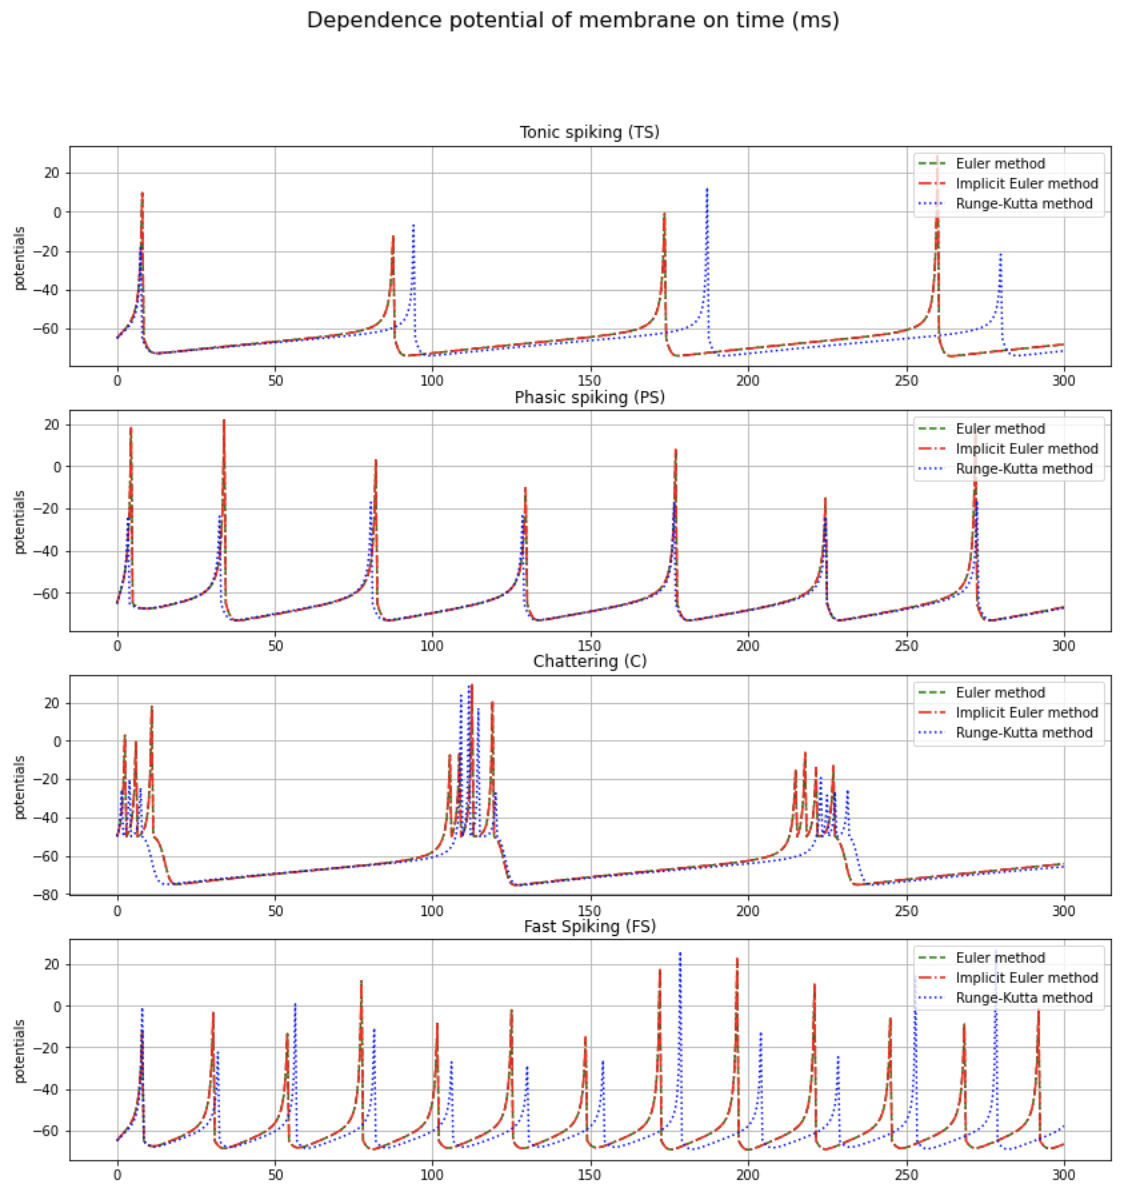
\includegraphics[scale=0.75]{traek1}}
\caption{Траектории динамических систем для соответствующих режимов и методов}
\end{figure}
\subsubsection{Особенности режимов}
\hspace*{\parindent}Как видно из рисунка (\hyperlink{res4}{1}), каждый из режимов отличен друг от друга.\\
\indentДля режима \textit{Tonic spiking} характерны 2 импульса, между которыми происходит длительное восстановление мембраны. Особенность данного режима по сравнению с другими - длительное восстановление мембраны.\\ 
\indentДля режима \textit{Phasic spiking} характерно, в сравнении с предыдущем, что количество импульсов увеличилось, а длительность восстановления мембраны уменьшилась.\\ 
\indentДля режима \textit{Chattering} видно, что происходит три импульса подряд, между которыми восстановление мембраны происходит практически мгновенно, а затем следует длительное восстановление мембраны. Особеность режима \textit{Chattering} заключается в нескольких подряд идущих импульсах, между которыми восстановление мембраны происходит быстро, а затем, после этих импульсов - длительное восстановление мембраны.\\ \indentДля режима \textit{Fast Spiking} заметно, что количество импульсов, в сравнении с другими режимами, - максимально, а средняя длительность восстановления мембраны - минимальна.
\subsection{Моделирование Нейронной сети}
\subsubsection{Сравнение методов Эйлера (явный/неявный) и метода Рунге-Кутта}
\hspace*{\parindent}Как уже было сказано ранее - неявный метод Эйлера - небольшая модификация явного метода Эйлера. Неявные методы в общем случае всегда дают более точный результат, чем явные методы, для одного и того же количества шагов или вычислений функции. Ключевое отличие их заключается в том, что неявный метод Элейра является \texit{абсолютно устойчивым}, в то время как явный - лишь условно устойчивый. Так как точность метода определяется отброшенными членами ряда, то согласно (\hyperlink{res1}{6}), метод Эйлера имеет порядок точности $\approx  h^2$. \\
\indent Самое большое распространение из всех численных методов решения дифференциальных уравнений с помощью ЭВМ получил метод Рунге-Кутта 4-го порядка. В литературе он известен как метод Рунге-Кутта. Отметим, что метод Рунге-Кутта 2-го порядка так же называют модифицированным методом Эйлера.
\begin{equation}
    w_0 = \alpha, 
    w_{i+1} = w_i + hf(t_i + \frac{h}{2}, w_i+\frac{h}{2}f(t_i,w_i))
\end{equation}
\indent Метод Рунге-Кутта 4-го порядка, имеет больший порядок точность чем метод Эйлера ($\approx h^4$), однако он является алгебраически более трудоемким. Явный метод Рунге-Кутта так же является условно-устойчивым (неявный - абсолютно устойчивый)\\
\indentТаким образом, Метод Эйлера (явный/неявный), классический Метод Рунге-Кутта - это численные методы получения решения дифференциальных уравнений. Они различаются порядком точности, степенью устойчивости и сложностью алгебраического воспроизведения (т. е. фактически - сложностью реализации и кол-во требуемых выч. ресурсов).
\subsubsection{Моделирование во времени нейронной сети с помощью метода Эйлера}
\hspace*{\parindent}Необходимо с помощью заданной модели Ижикевича смоделировать динамику нейронной сети, состоящей из 1000 нейронов - 800 возбуждающих, 200 - тормозных.
\indentПрежде чем осуществлять непосредственное моделирование - необходимо произвести первичную инициализацию нейронов и их параметров. Кроме того, необходимо создать и проинициализировать весовую матрицу смежности \textbf{W} - матрицу внешних токов, при появлении в сети импульса.
Так же требуется, с помощью начальных параметров задать временную сетку: \\
\begin{equation*}
    h1 = (t_n_1-t_0_1)/(len(t_1)-1)
\end{equation*}

Приведем программную реализацию вышеперечисленного:\\
\textbf{Листинг 6. Инициализация необходимых параметров}
\hypertarget{lst6}{}
\begin{python}
W_matrix = np.zeros((1000, 1000))
for i in range (0, 1000):
  for j in range (0,800):
    if i != j:
      W_matrix[i][j] = 0.5 * np.random.uniform()
  for j in range (800, 1000):
    if i != j:
      W_matrix[i][j] = -np.random.uniform()

params_neurons = [{'a' : 0 , 'b' : 0,'c' : 0, 'd' : 0, 'I' : 0, 'id' : 0} for i in range (1000)]
id = 1

for i in range (800):
  params_neurons[i]['a'] = 0.02
  params_neurons[i]['b'] = 0.2
  params_neurons[i]['c'] = -65 + 15 * np.random.uniform() ** 2
  params_neurons[i]['d'] = 8 - 6 *  np.random.uniform() ** 2
  params_neurons[i]['I'] = 5 * np.random.uniform() 
  params_neurons[i]['id'] = id
  id += 1

for i in range (800, 1000):
  params_neurons[i]['a'] = 0.02 + 0.08 * np.random.uniform()
  params_neurons[i]['b'] = 0.25 - 0.05 * np.random.uniform()
  params_neurons[i]['c'] = -65 
  params_neurons[i]['d'] = 2 
  params_neurons[i]['I'] = 2 * np.random.uniform() 
  params_neurons[i]['id'] = id
  id += 1

t_1 = np.linspace(0, 1000, 21)
t_0_1 = 0
t_n_1 = 1
h1 = (t_n_1-t_0_1)/(len(t_1)-1)
increased_current = np.zeros((len(t_1), 1000))
\end{python}
\indentКак можно видеть из Листинга (\hyperlink{lst6}{6}), моделирование автором производится на промежутке от 0 до 1000 мс, с шагом 50 мс. \\
\indentДалее автором вводится понятие - $"$вспомогательные параметры$"$ - это фактически параметры нейрона, рассматриваемого в данный момент времени. Необходимость ввода таких параметров обусловена сугубо удобством автора. \\
Дальнейшая реализация сводится к следующему алгоритму:
\begin{enumerate}
    \item Производится первичная инициализация нулями двумерной матрицы \textit{increased_current} - содержащей значения токов нейронов в случае возникновения импульса.
	\item Производится инициализация вспомогательных параметров параметрами конкретного нейрона.
    \item Вспомогательный ток инициализируется либо соответствующим элементом матрицы \textit{increased_current} (если ранее был импульс и там не ноль), либо базовым током рассматриваемого нейрона.
    \item Далее в цикле рассматривается конкретный нейрон во всех промежутках времени, если на каком из промежутков был импульс - выводятся номер нейрона, временной промежуток и значение потенциала; соответствующие элементы матрицы \textit{increased_current} увеличиваются согласно условию (ток от нейрона с импульсом передается другим нейронам)
    
\end{enumerate}
\indentМодель нейронной сети выводится как в трех-мерном представлении, так и в двух-мерном представлении. \\
Представим программную реализацию вышенаписанного алгоритма. \\
\textbf{Листинг 7. Моделирование нейронной сети в 3-х мерном пространстве}
\hypertarget{lst10}{}
\begin{python}
fig = plt.figure(figsize=(14, 10))
ax_3d = Axes3D(fig)
ax_3d.set_xlabel('time (ms)', fontsize = 15)
ax_3d.set_ylabel('neuron id', fontsize = 15)
ax_3d.set_zlabel('V', fontsize = 17)
I = [0 for c  in range (len(t_1))]
increased_current = np.zeros((len(t_1), 1000))
for i in range (0, 1000):
    a = params_neurons[i]['a']
    b = params_neurons[i]['b']
    c = params_neurons[i]['c']
    d = params_neurons[i]['d']
    for k in range (len(t_1)):
      if increased_current[k][i] == 0:
        I[k]  = params_neurons[i]['I']
      else:
        I[k] = increased_current[k][i]
    id = params_neurons[i]['id']
    v = mod_euler(t_0_1, t_n_1, [f1, f2], h1, I)
    for p in range (len(v)):
      if v[p] == c:
        for j in range (1000):
          increased_current[p][j] = increased_current[p][j] + params_neurons[j]['I'] +  W_matrix[j][i]
        if (i+1 <= 800):
          _ = ax_3d.scatter(t_1[p], i+1, v[p], color = 'red')
        else: 
          __ = ax_3d.scatter(t_1[p], i+1, v[p], color = 'blue')
ax_3d.set_title("Neural network modeling (3D)", loc='center', fontsize = 25)
_.set_label('Excitatory neuron')
__.set_label('Inhibitory neuron')
plt.legend(fontsize = 14)
plt.show()
\end{python}
\indent Моделирование в 2-х мерном пространстве по своей сути аналогично 3-х мерному, поэтому для большей лаконичности изложения, приводиться не будет. \\
Согласно Листингу (\hyperlink{lst10}{7}) изобразим моделирование нейронной сети в 3-х мерном пространстве. 
\hypertarget{3d}{}
\begin{figure}[h!]
\center{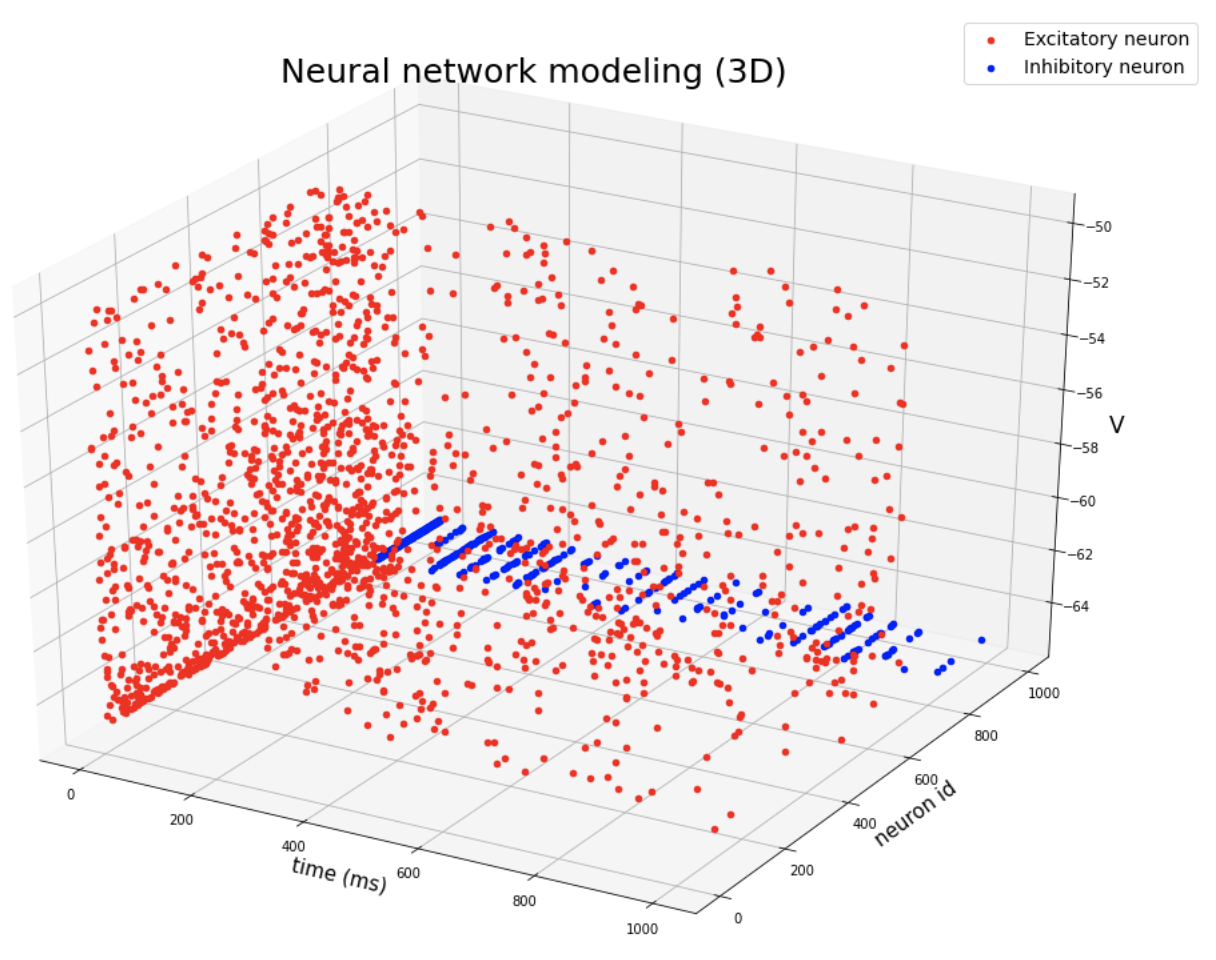
\includegraphics[scale=0.55]{3d}}
\caption{Моделирование импульсов нейронов в трехмерном представлении. Красный цвет - возбуждающий нейрон, синий - тормозной нейрон.}
\end{figure}
\clearpage
\indentТеперь, приведем моделирование нейронной сети в 2-х мерном пространстве. Оси абсцисс будет соответствовать $id$ нейрона, оси ординат - временной момент моделирования. Точка соответствует случившемуся импульсу данного нейрона. \\
\hypertarget{2d}{}
\begin{figure}[h!]
\center{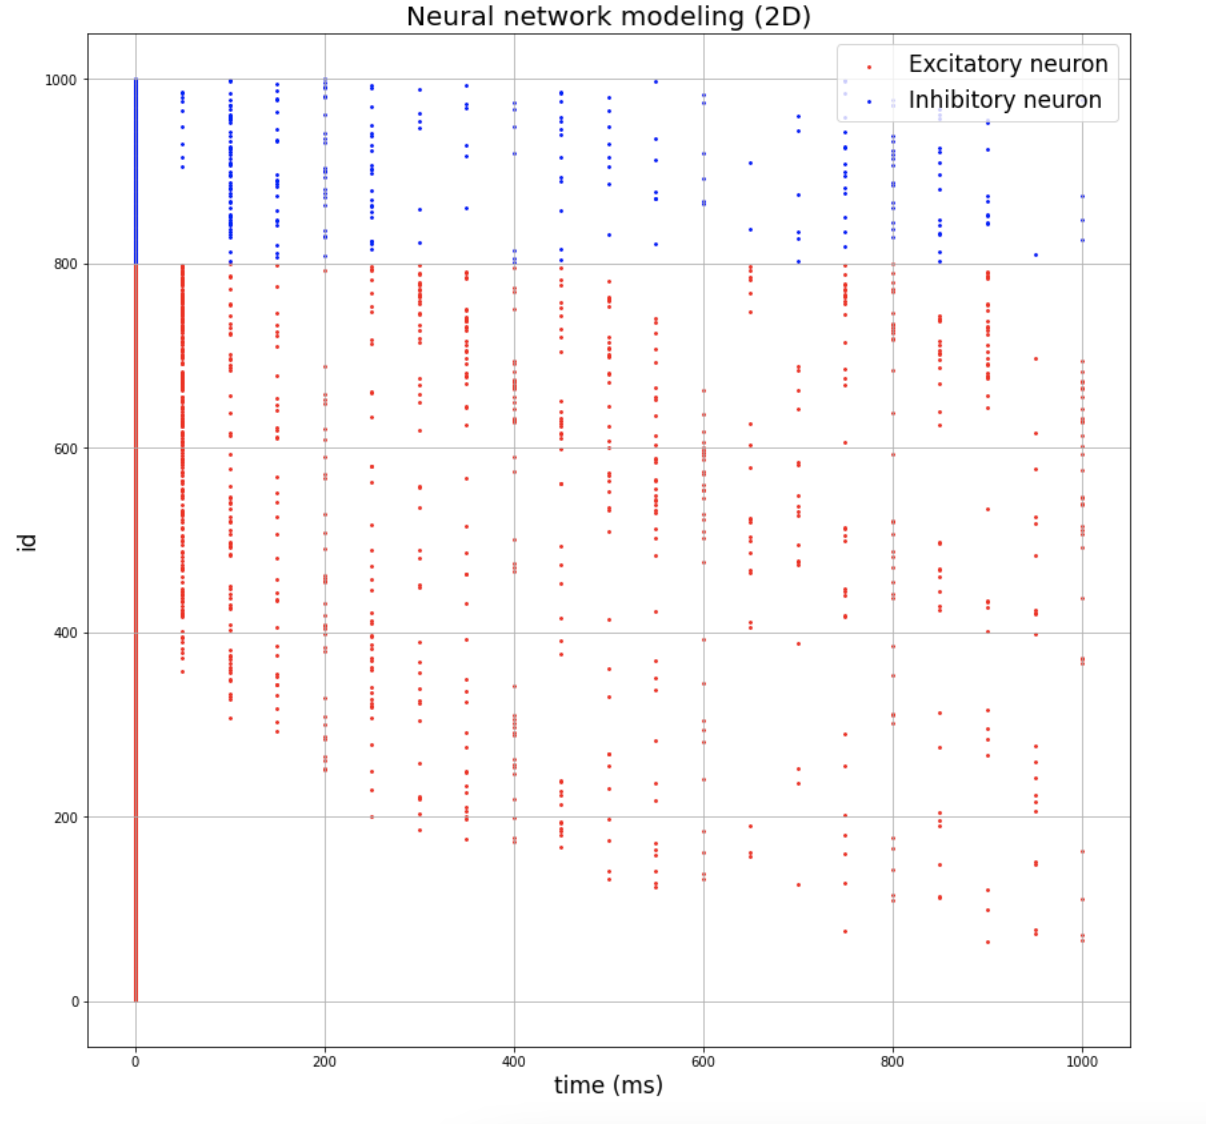
\includegraphics[scale=0.6]{2d}}
\caption{Моделирование импульсов нейронов в двухмерном представлении. Красный цвет - возбуждающий нейрон, синий - тормозной нейрон. Точка - импульс.}
\end{figure}

\indentСудя по полученным графикам (\hyperlink{3d}{2}), (\hyperlink{2d}{3}), заметим, что колебания являются частично синхронными - все зависит от сгенерированных параметров нейрона и, следовательно, - от его типа. Так, например, очевидно, что для возбуждающего нейрона возникновение импульса - гораздо характернее, чем для тормозного нейрона. \\
\indent Тем не менее, примерная частота полученных колебаний составляет 10-15 Гц. 
\clearpage
\subsection{Заключение}
\begin{enumerate}
\item Проведена реализация численных методов решения задачи Коши - явный метод Эйлера, неявный метод Эйлера, метод Рунге-Кутта.
\item С помощью вышеперечисленных методов были построены траектории динамических систем для соответствующего режима работы Нейрона.
\item Произведено моделирование нейронной сети, состоящей из 1000 нейронов - 800 возбуждающих, 200 тормозных.
\item Получена графическая интерпретация моделирования как в 3-х мерном пространстве, так и в 2-х мерном пространстве.
\item Определен тип колебаний импульсов нейронов - частичные колебания. Определена примерная частота полученных колебаний - 10-15 Гц.
\end{enumerate}
\hspace*{\parindent}В совокупности, данная лабораторная работа позволила лучше понять и проработать материал, связанный с понятиями: модель Ижикевича, задача Коши, явный метод Эйлера, неявный метод Эйлера, Методы Рунге-Кутта, флуктуации, возбуждающий нейрон, тормозной нейрон.

%----------------------------------------------------------
\subsubsection*{Список использованных источников}

\begin{enumerate}
	\item \bibentry{Pershin2018CompMath}
    \item \textrm{[Электронный ресурс]} Першин А. Ю. Видео-лекции по курсу "Вычислительная математика". Москва, 2021
    \textit{https://www.youtube.com/channel/UC69GDhPVLY_7IXn3EhmcH2w}
\end{enumerate}

%----------------------------------------------------------
\subsubsection*{Выходные данные}

\textit{\DocOutReference}
%----------------------------------------------------------
% Атрибуты задачи
\labattributes{}{}{}{}{студент группы \EduGroup, \Author}{\Year, \Semestr}
%----------------------------------------------------------

